\chapter{Model grafowy problemu zakupu licencji}

\section{Reprezentacja grafowa}

Aby formalnie opisać zjawisko współdzielenia licencji, sieć relacji społecznych modelujemy jako graf nieskierowany \( G = (V, E) \). Każdy wierzchołek \( v \in V \) reprezentuje pojedynczego użytkownika, natomiast krawędź \( \{u, v\} \in E \) oznacza, że użytkownicy \( u \) i \( v \) znajdują się w relacji umożliwiającej współdzielenie licencji grupowej. Graf jest nieskierowany, ponieważ zakładamy symetryczność tej relacji: jeśli \( u \) zna \( v \), to również \( v \) zna \( u \).

Przyjmujemy również, że graf \( G \) nie zawiera pętli, tj. \( \{v, v\} \notin E \) dla każdego \( v \in V \), ani krawędzi wielokrotnych - każda para użytkowników może być powiązana co najwyżej jedną krawędzią. Przykład takiej struktury zilustrowano na Rysunku \ref{fig:social_graph}.

\begin{figure}[H]
    \centering
    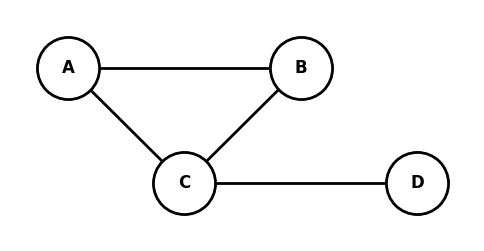
\includegraphics[width=0.5\textwidth]{assets/graphmodelexample.png}
    \caption{Przykładowy graf relacji społecznych między użytkownikami.}
    \label{fig:social_graph}
\end{figure}

Opisana reprezentacja, w której wierzchołki odpowiadają jednostkom, a krawędzie bezpośrednim relacjom umożliwiającym interakcję, jest powszechnie stosowana w analizie sieci społecznościowych \cite{Brandes2004, NETTLETON20131}. Takie ujęcie pozwala formalnie modelować i badać zjawiska zachodzące w społecznościach użytkowników usług cyfrowych.

„W przyjętym modelu zakłada się, że współdzielenie licencji może odbywać się wyłącznie między osobami połączonymi bezpośrednią krawędzią w grafie. Licencja grupowa oznacza w tym kontekście typ umożliwiający współdzielenie dostępu przez właściciela oraz jego bezpośrednich sąsiadów. Oznacza to, że użytkownicy muszą znać się bezpośrednio i mieć wzajemne zaufanie, co jest istotne na przykład w przypadku przekazywania danych logowania lub zapraszania do planu rodzinnego. Relacje pośrednie, w których użytkownicy są powiązani poprzez wspólnych znajomych (np. \( A \sim B \) oraz \( B \sim C \), lecz brak bezpośredniego powiązania \( A \sim C \)), nie są uwzględniane w analizie. Oznacza to, że dla danego grafu \( G = (V, E) \),
w którym \( V \) to zbiór użytkowników, a \( E \subseteq \{ \{u,v\} : u,v \in V, u \neq v \} \) to zbiór relacji znajomości, analizie podlegają wyłącznie relacje bezpośrednie, czyli pary \( \{u, v\} \in E \).
Na przykład w grafie przedstawionym na Rysunku \ref{fig:social_graph}, użytkownicy \( A \) i \( D \) są wprawdzie połączeni za pośrednictwem ścieżki \( A \rightarrow C \rightarrow D \), jednak ponieważ brakuje bezpośredniego połączenia \( \{A,D\} \in E \), to taka relacja nie jest uznawana za podstawę do współdzielenia licencji w tym modelu.
Mimo że w praktyce relacje pośrednie - takie jak ścieżki długości większej niż jeden - mogą sprzyjać tworzeniu grup subskrypcyjnych, w analizie zostały one pominięte w celu uproszczenia problemu.

Graf społecznościowy nie musi być pełny - dopuszcza się dowolną strukturę odpowiadającą rzeczywistym relacjom społecznym. W analizie istotną rolę odgrywa stopień wierzchołków, ponieważ decyduje on o liczbie osób, którym dany użytkownik może udostępnić swoją licencję. Dla wierzchołka \( v \in V \), jego stopień oznaczamy przez \( \deg(v) \), co odpowiada liczbie sąsiadów użytkownika \( v \) w grafie \( G = (V, E) \).

Należy jednak zauważyć, że nawet w przypadku wysokiego stopnia $\deg(v)$, użytkownik niekoniecznie może współdzielić licencję ze wszystkimi swoimi sąsiadami. Ograniczenia techniczne, takie jak limity liczby współużytkowników narzucane przez dostawcę usługi, sprawiają, że liczba osób objętych jedną licencją grupową pozostaje ograniczona. W analizowanym modelu wprowadzamy zatem parametr $k$, oznaczający pojemność licencji grupowej, czyli maksymalną liczbę osób, wliczając w to właściciela, które mogą korzystać z jednej licencji.



\section{Definicja problemu}\label{sec:model-formal}

Optymalizacja kosztu dostępu do usługi wymaga przypisania wszystkim wierzchołkom grafu $G ~=~ (V,~E)$ odpowiednich ról. Każdy użytkownik $v \in V$ może uzyskać dostęp do usługi na trzy sposoby:
\begin{enumerate}
    \item Poprzez wykupienie licencji indywidualnej.
    \item Poprzez wykupienie licencji grupowej.
    \item Jako odbiorca, korzystający z licencji grupowej należącej do innego użytkownika.
\end{enumerate}
Licencja indywidualna zapewnia dostęp wyłącznie jej właścicielowi, natomiast licencja grupowa umożliwia współdzielenie dostępu z maksymalnie $k-1$ sąsiadami w grafie.

Dla przejrzystego i precyzyjnego zdefiniowania modelu wprowadzamy trzy zbiory reprezentujące użytkowników, czyli węzły posiadające własną licencję bądź korzystające z licencji innego węzła:
\begin{itemize}
  \item $I$ - posiadacze licencji indywidualnych;
  \item $G$ - posiadacze licencji grupowych;
  \item $R$ - odbiorcy, którzy sami nie kupują licencji, lecz korzystają z licencji innego użytkownika.
\end{itemize}

Aby formalnie opisać ten podział, wprowadzamy etykietowanie ról $f:V\to\{0,1,2\}$.
Wartość $0$ oznacza węzeł będący odbiorcą, $1$ odpowiada licencji indywidualnej, a $2$ licencji grupowej.
Takie przypisanie nawiązuje do klasycznego problemu dominowania rzymskiego, w którym wierzchołki również otrzymują etykiety z tego samego zbioru wartości.
Odpowiadające zbiory definiujemy jako $I=\{v:f(v)=1\}$, $G=\{v:f(v)=2\}$ oraz $R=V\setminus(I\cup G)$.
Przyjmujemy zbiór dostępnych typów licencji
\begin{equation}
  \mathcal{L} = \{ \ell_t = (c_t, m_t, k_t) \mid t = 1,2,\dots,T \},
  \label{eq:license_family}
\end{equation}
gdzie:
\begin{itemize}
  \item $c_t$ - koszt licencji typu $t$,
  \item $m_t$ — minimalna liczba użytkowników wliczając właściciela,
  \item $k_t$ — maksymalna liczba użytkowników wliczając właściciela,
  \item $T$ — całkowita liczba dostępnych typów licencji.
\end{itemize}
W podstawowym wariancie rozważanym w tym rozdziale zakładamy, że zbiór $\mathcal{L}$ opisany we wzorze~(\ref{eq:license_family}) obejmuje wyłącznie dwa typy licencji: indywidualną oraz jedną grupową, a zatem przyjęte jest $T = 2$. Model ten nie przewiduje sytuacji z wieloma rodzajami planów grupowych (np. Duo, Family), lecz ogranicza się do najprostszego przypadku odpowiadającego rozwiązaniom takim jak w Duolingo.

\paragraph{Warunki wykonalności.}
Spełnienie rozwiązania wymaga, aby dla etykietowania $f:V\to\{0,1,2\}$ zachodziły następujące warunki:
\begin{enumerate}
  \item Pokrycie: Każdy użytkownik $v \in V$ musi mieć dostęp do usługi, tj. $f(v)\in\{1,2\}$ lub istnieje sąsiad $u\in N(v)$ taki, że $f(u)=2$ i $v$ jest przypisany do grupy $u$.
  \item Sąsiedztwo: Odbiorca $v\in R$ może być przypisany tylko do właściciela $u\in G$ z $\{u,v\}\in E$.
  \item Pojemność: Liczba użytkowników przypisanych do właściciela $u\in G$ (wraz z nim samym) musi spełniać $m \le 1+|R_u| \le k$, gdzie $R_u$ oznacza zbiór odbiorców korzystających z licencji $u$.
\end{enumerate}


\paragraph{Funkcja kosztu.}
W wariancie podstawowym, w którym $T=2$, całkowity koszt rozwiązania wyraża się zależnością:
\begin{equation}
  \cost(f) = |I|\cdot c_i + |G|\cdot c_g ,
  \label{eq:cost_function}
\end{equation}
gdzie:
\begin{itemize}
  \item $I$ - zbiór użytkowników z licencją indywidualną,
  \item $G$ - zbiór użytkowników z licencją grupową,
  \item $c_i$ - koszt licencji indywidualnej,
  \item $c_g$ - koszt licencji grupowej.
\end{itemize}

\paragraph{Cel optymalizacji.}
Celem problemu jest minimalizacja funkcji kosztu~(\ref{eq:cost_function}) dla danego grafu $G=(V,E)$, przy spełnieniu wszystkich istotnych warunków wykonalności.


% Odpowiadający problem decyzyjny polega na sprawdzeniu, czy istnieje taki wybór zbiorów $I$ i $G$, że spełnione są wszystkie warunki oraz zachodzi nierówność:
% \[
% |I| + p \cdot |G| \leq K,
% \]
% dla danego ograniczenia kosztowego $K$.

\section{Koszty i ograniczenia}

\subsection{Ograniczenia techniczne i społeczne współdzielenia licencji}

Kluczowymi parametrami modelu są minimalna oraz maksymalna liczba osób, które mogą współdzielić jedną licencję grupową. Maksymalny rozmiar grupy oznaczamy przez $k$ i wliczamy do niego także użytkownika nabywającego licencję. Parametr $k$ jest zwykle narzucany przez dostawcę usługi. Przykładowo, plan rodzinny Spotify Premium pozwala na korzystanie maksymalnie sześciu osobom (właściciel + pięć członków rodziny), co odpowiada wartości $k=6$.

Analogicznie wprowadzamy parametr $m$, który określa minimalną liczbę osób niezbędnych do utworzenia grupy. Oznacza to, że licencja grupowa jest ważna tylko wtedy, gdy zostanie wykorzystana przez co najmniej $m$ osób (łącznie z właścicielem). Przykładem jest tzw. plan „Duo”, w którym licencję mogą współdzielić dokładnie dwie osoby ($m=2, k=2$). W innych przypadkach $m$ może przyjmować wartości mniejsze niż $k$, np. $m=2, k=6$ dla planów rodzinnych.

W analizie przyjmujemy $m$ oraz $k$ jako zmienne parametry. Nawet jeśli użytkownik posiada wielu znajomych (czyli ma wysoki stopień w grafie), ograniczenie $k$ sprawia, że może objąć współdzieleniem tylko określoną maksymalną liczbę osób, natomiast ograniczenie $m$ wymusza, by grupy nie były zbyt małe. Parametry te modelują zarówno ograniczenia techniczne narzucane przez dostawców usług, jak i czynniki społeczne, takie jak opłacalność czy gotowość do współdzielenia subskrypcji. W konsekwencji grupy współdzielenia odwzorowują typowe sytuacje, w których w praktyce licencje grupowe są wykorzystywane.


% \subsection{Struktura kosztów i modele cenowe}

% Przyjmujemy, że koszt licencji indywidualnej wynosi $1$ jednostkę, natomiast koszt licencji grupowej oznaczamy przez $p$. W rzeczywistych ofertach wartość $p$ różni się w zależności od usługi, lecz zazwyczaj jest mniejsza niż suma kosztów indywidualnych licencji dla wszystkich użytkowników planu, co stanowi zachętę do współdzielenia. W szczególności interesujące są przypadki, gdy $p < k$, ponieważ wtedy koszt jednostkowy w planie grupowym, równy $p/k$, jest niższy niż $1$.

% Jeżeli natomiast $p = k$, oznaczałoby to brak korzyści ze współdzielenia - koszt na osobę byłby identyczny jak w przypadku zakupu licencji indywidualnej. W praktyce jednak zazwyczaj zachodzi $p < k$, a często nawet $p \ll k$, co czyni współdzielenie ekonomicznie korzystnym.

% Do zilustrowania różnych scenariuszy rozważane będą miedzy innymi poniższe modele cenowe:
% \begin{enumerate}
%     \item \textbf{Model A}: $p=2$, $k=5$ - licencja grupowa dwukrotnie droższa od indywidualnej, obejmująca pięć osoby,
%     \item \textbf{Model B}: $p=3$, $k=5$ - licencja grupowa trzykrotnie droższa od indywidualnej, również obejmująca pięć osób.
% \end{enumerate}
% Zarówno model A jak i model B reprezentują rzeczywisty rozmiar ilości osób mogących korzystać z jednej zakupionej licencji grupowej. Istotną różnicą jest tutaj cena obu tych przypadków. Interesujący może być wpływ ceny na ilość występowania zakupionych licencji indywidualnych oraz grupowych w porównaniu modeli o różnych wartości obu tych licencji.

\subsection{Struktura kosztów i modele cenowe}

W analizowanym problemie istotnym elementem jest sposób odwzorowania polityki cenowej dostawców usług.
Różne plany subskrypcyjne charakteryzują się nie tylko innym kosztem, ale również odmiennym zakresem liczby użytkowników $k$, którzy mogą korzystać z jednej licencji.
Dodatkowo wprowadzane jest ograniczenie dolne $m$, które definiuje minimalną liczbę użytkowników planu.
Mimo że w rzeczywistości takie ograniczenia nie są formalnie narzucane, w prezentowanym modelu pełnią ważną rolę, gdyż odzwierciedlają ekonomiczny sens wyboru licencji grupowych.
W praktyce bowiem korzystanie z planu grupowego przez jedną osobę jest nieopłacalne.
Przykładowo, dla planów typu Duo czy Family naturalne jest przyjęcie $m=2$, mimo że technicznie możliwe byłoby używanie takiej subskrypcji w pojedynkę.
Rodzinę typów licencji zdefiniowaną we wzorze~\eqref{eq:license_family} stosujemy tutaj do opisu struktury kosztów i ograniczeń dostępnych planów.
W testach syntetycznych wartości parametrów licencji dobierane są eksperymentalnie, co pozwala badać zachowanie algorytmów w różnych wariantach cenowych i strukturalnych.
W testach na danych rzeczywistych wykorzystywane są faktyczne ceny subskrypcji.
Dla wariantu teoretycznego odpowiadającego dominacji rzymskiej koszty normalizowane są względem licencji indywidualnej, co umożliwia powiązanie modelu z klasycznymi zagadnieniami teorii grafów.
Przykłady zestawiono w~Tabeli~\ref{tab:license_models_real}.


\begin{table}[h!]
\centering
\caption{Przykładowe modele licencji dla usług rzeczywistych i modelu teoretycznego}
\begin{tabular}{lccc}
\hline
\textbf{Typ licencji} & \textbf{Koszt $c_t$} & \textbf{Min $m_t$} & \textbf{Max $k_t$} \\
\hline
\multicolumn{4}{c}{\textit{Spotify (ceny w PLN)}} \\
Individual & 23,99 & 1 & 1 \\
Duo        & 30,99 & 2 & 2 \\
Family     & 37,99 & 2 & 6 \\
\hline
\multicolumn{4}{c}{\textit{Netflix (ceny w PLN)}} \\
Basic       & 33,00 & 1 & 1 \\
Standard    & 49,00 & 1 & 2 \\
Premium     & 67,00 & 1 & 4 \\
\hline
\multicolumn{4}{c}{\textit{Duolingo Super (ceny w PLN)}} \\
Individual & 13,99 & 1 & 1 \\
Family     & 29,17 & 2 & 6 \\
\hline
\multicolumn{4}{c}{\textit{Model teoretyczny (koszty znormalizowane)}} \\
Solo       & 1,0   & 1 & 1 \\
Group      & 2,0   & 2 & 999999 \\
\hline
\label{tab:license_models_real}
\end{tabular}

Źródło: opracowanie własne modelu teoretycznego oraz \cite{spotify_price2024}, \cite{spotify_price2025}, \cite{duolingo_app2024}.

\end{table}


W przypadku usług rzeczywistych koszty planów grupowych są znacznie niższe niż suma odpowiadających im licencji indywidualnych. Na przykład plan Spotify Family pozwala na współdzielenie subskrypcji przez maksymalnie sześć osób przy koszcie $37{,}99$ PLN, co czyni go zdecydowanie bardziej opłacalnym od planu indywidualnego ($23{,}99$ PLN). Podobna sytuacja występuje w przypadku Duolingo Super Family.

W modelu teoretycznym opartym na dominacji rzymskiej koszty są podane w jednostkach względnych. Licencja indywidualna ma koszt $1.0$, a licencja grupowa koszt $2.0$, co odpowiada klasycznemu przypisaniu wag w problemie dominacji rzymskiej. W ramach przeprowadzanych eksperymentów etykieta „2” będzie zmieniała swoją wartość jako wielokrotność kosztu ceny indywidualnej, co pozwala na analizę różnych wariantów tego zagadnienia.


% \subsection{Zakup jednoczesny i sekwencyjny}

% W podstawowej wersji problemu zakłada się, że decyzje zakupowe wszystkich użytkowników są podejmowane jednocześnie, co umożliwia globalną optymalizację. W praktyce jednak proces współdzielenia często przebiega dynamicznie. Najpierw pewne grupy użytkowników kupują licencje indywidualnie, a dopiero później tworzą grupy współdzielenia.

% Taki dynamiczny scenariusz można modelować jako proces wieloetapowy, w którym w kolejnych krokach następuje przydział użytkowników do nowych licencji. Warto zauważyć, że rozwiązanie optymalne przy jednoczesnym zakupie może być trudne do osiągnięcia w procesie sekwencyjnym. Decyzje podejmowane wcześniej mogą ograniczać dostępne opcje w kolejnych etapach.

% W pracy omówione zostaną wyzwania związane z rozwiązaniami sekwencyjnymi, takie jak stabilność struktur współdzielenia czy mechanizmy motywujące do współpracy. Główny nacisk kładziony jest jednak na analizę wariantu jednoczesnego, który umożliwia zastosowanie klasycznych narzędzi teorii grafów i optymalizacji dyskretnej, oraz stanowi punkt odniesienia dla bardziej złożonych scenariuszy dynamicznych.

\subsection{Zakup jednoczesny i sekwencyjny}

W najprostszym wariancie zakłada się, że wszystkie decyzje zakupowe zapadają w tym samym momencie. Umożliwia to globalną optymalizację i stanowi punkt odniesienia dla analiz teoretycznych. W praktyce jednak proces współdzielenia licencji jest bardziej dynamiczny. Użytkownicy dołączają do planów w różnych chwilach, część początkowo wybiera licencje indywidualne, a dopiero później postanawia zakupić subskrypcję grupową. Takie zmiany licencji mogą również wynikać z równoczesnej zmiany i ewolucji sieć społecznościowej w czasie rzeczywistym. Relacje znajomości mogą zanikać, powstawać mogą nowe połączenia, a liczba aktywnych użytkowników zmienia się w czasie.

Takie sytuacje można modelować jako proces sekwencyjny, w którym w kolejnych krokach przydzielane są nowe licencje przy uwzględnieniu bieżącej struktury grafu. Prowadzi to do odmiennych trudności niż w przypadku wariantu uproszczonego, czyli jednoczesnego. Rozwiązanie optymalne globalnie może okazać się nieosiągalne, ponieważ wcześniejsze decyzje oraz zmiany w strukturze sieci ograniczają przestrzeń dostępnych opcji w późniejszych etapach.

W pracy przeanalizowane zostały konsekwencje tego typu dynamicznych zmian takie jak stabilność i trwałość powstałych grup, wpływ zmian w grafie na opłacalność wcześniejszych decyzji, a także mechanizmy sprzyjające koordynacji i adaptacji użytkowników. Mimo że główny nacisk położony jest na wariant jednoczesny, wariant sekwencyjny stanowi istotne rozszerzenie modelu i lepiej odzwierciedla rzeczywiste warunki funkcjonowania sieci społecznościowych.
